\chapter{Μετρήσεις και Επίδειξη Εφαρμογής}
\label{chapter:system_showcase}

Στο κεφάλαιο αυτό θα μελετήσουμε την απόδοση του συστήματος Lychte που υλοποιήσαμε στο πλαίσιο της διπλωματικής
αυτής εργασίας και, στο τέλος, θα παρουσιαστούν εικόνες από τη γραφική διεπαφή, την εφαρμογή δηλαδή που αναπτύξαμε.

\section{Μετρήσεις}
\label{section:expreriments}

Προκειμένου να παρακολουθήσουμε τις ανάγκες και να δοκιμάσουμε τα όρια του Lychte καναμε μία σειρά διαφορετικών μετρήσεων. Η παράμετρος
που αλλάζει σε κάθε μέτρηση είναι ο αριθμός των Apis/Jobs που τρέχει παράλληλα ένας worker. Έτσι σε κάθε διαφορετική μέτρηση
κάναμε $n$ καταχωρήσεις Apis και Jobs αντίστοιχα, όπου $n$ o αρθμός των αιτημάτων που θέλουμε να ελέγχουμε. Στο σημείο αυτό πρέπει να ανεφερθεί
ότι οι μετρήσεις έγιναν σε μηχάνημα με τα εξής τεχνικά χαρακτηριστικά:

\begin{table}[H]
	\begin{center}
		\caption{Τεχνικά χαρακτηριστικά Υπολογιστικού Συστήματος}
		\label{tab:pc_specs}
		\begin{tabular}{| c | c |}
			\hline
			\thead{Operating System} & WindowsOS                  \\
			\hline
			\thead{Processor}        & AMD Ryzen 7 5800H (3,2Ghz) \\
			\hline
			\thead{RAM}              & 16GB                       \\
			\hline
		\end{tabular}
	\end{center}
\end{table}

\newpage

\subsection{Περιγραφή}
\label{subsection:experiment_summary}

Προκειμένου να κάνουμε τις μετρήσεις χρειαζόμαστε κάποια urls τα οποία θα πρέπει να καλούμε ανά τακτά χρονικά διαστήματα, αυτά που κανονικά ορίζει ο χρήστης
κατά τη διαδικασία δημιουργίας ενός Api. Για να υπάρχει μία ποικιλία στο πλήθος των ιστοσελιδών και διαδικτυακών apis που παρακολουθούμε και να μελετήσουμε τη λειτουργία του Lychte σε
μία κατάσταση όσο το δυνατό πιο κοντά σε πραγματικά σενάρια, δημιουργήσαμε script που γράφει με τυχαίο τρόπο $n$ Apis και Jobs, στα αντίστοιχα collections της βάσης, έχοντας μία προκαθορισμένη
λίστα urls, μαζί με στοιχεία που ίσως χρειάζονται για αυθεντικοποίηση (tokens). Μαλιστα, για να ελέγξουμε τη σταθερότητα του συστήματος ως προς
το χρόνο μεταξύ των διαδοχικών αιτημάτων ενός Api για διάφορους χρονισμούς, περά από την τυχαιότητα επιλογής του συνδέσμου στον οποίο θα κάνουμε κλήσεις
επιλέγεται με τυχαίο τρόπο και ο χρόνος μεταξύ των αιτημάτων (τo interval κάθε Αpi/Job). Επειδή σκοπός των μετρήσεων που κάναμε είναι
το stress test του συστήματος, οι χρόνοι που επιλέχθηκαν είναι ένας μεταξύ των τριάντα δευτερολέπτων, ενός, δύο, ή τριών λεπτών.

Πιο συγκεκριμένα τα σενάρια που δοκιμάστηκαν είναι τα εξής:
\begin{itemize}
	\item $n = 100$ apis
	\item $n = 500$ apis
	\item $n = 1.000$ apis
	\item $n = 5.000$ apis
\end{itemize}

Κάθε μία από τις παραπάνω διαφορετικές μετρήσεις διήρκησε δώδεκα ώρες. Σε αυτό το μήκος χρόνου, 
μετρήθηκαν η μέση χρήση/κατανάλωση CPU και RAM καθώς και η μέση απόκλιση του χρόνου μεταξύ των διάφορων διαδοχικών αιτημάτων
από τον αναμενόμενο, βάσει του interval κάθε Αpi, χρόνο που θα έπρεπε να ξαναεκτελεστεί. 

\subsection{Αποτελέσματα}
\label{subsection:experiment_results}

Στον \autoref{tab:results} μπορούμε να δούμε τα αποτελέσματα των μετρήσεών μας.

Παρατηρούμε ότι στα πρώτα τρία σενάρια η χρήση υπολογιστικών πόρων του συστήματος δεν είναι σημαντική, αλλά
και η μέση απόκλιση του χρόνου επανεκτέλεσης των Apis είναι πολύ μικρή. Μάλιστα παίρνει αρνητικές τιμές. Αυτό δεν οφείλεται σε κάποιο
λάθος στον υπολογισμούς μας, αλλά στον τρόπο λειτουργίας του scheduler. Για να κρίνει, αν πρέπει να εκτελέσει κάποιο αίτημα, έχει ένα μικρό bias
που του επιτρέπει να επιλέγει jobs που βρίσκονται πολύ κοντά στο χρόνο που πρέπει να ξανατρέξουν. H πόλωση αυτή του συστήματος είναι της τάξη
nano-δευτερολέπτων και έχει σκοπό να κερδίζει χρόνο για εξομαλύνει πιθανές καθυστερήσεις του συστήματος.  

Στην τελευταία σειρά μετρήσεων, που αφορά τα 5.000 apis, που εκτελούνται ταυτόχρονα από έναν και μόνο worker, μπορούμε εύκολα να δούμε ότι το σύστημα
συνεχίζει να ανταπεξέρχεται στις ανάγκες του ελέγχου και παρακολούθησης των apis του (μέσος χρόνος απόκλισης μικρότερος του δευτερολέπτου). Αξίζει να σημειωθεί,
όμως, όπως θα δούμε καλύτερα και στη συνέχεια ότι η κατανάλωση των υπολογιστικών πόρων είναι αρκετά μεγάλη, σε βαθμό μάλιστα που
ιδανικά θα κάναμε load balancing με έναν από δύο τρόπους. Μεταφέροντας τα αιτημάτα που εκτελεί σε έναν ή περισσότερους άλλους workers, ή βάζοντας άλλους workers να διαβάζουν
από το collection της υπό μελέτης διεργασίας.

\begin{table}[H]
	\begin{center}
		\caption{Αποτελέσματα Μετρήσεων}
		\label{tab:results}
		\begin{tabular}{| c | c | c | c |}
			\hline
			                  & \thead{Μέση Απόκλιση} & \thead{Μέση Χρήση CPU} & \thead{Μέση Χρήση RAM} \\
			\hline
			\thead{100 apis}  & -112,62ms             & 1,22\%                 & 102,54Mb               \\
			\hline
			\thead{500 apis}  & -69,32ms              & 3,26\%                 & 171,1Mb                \\
			\hline
			\thead{1.000 apis} & -47,9ms               & 7,46\%                 & 223,13Mb               \\
			\hline
			\thead{5.000 apis} & 664ms                 & 56,36\%                & 652,45Mb               \\
			\hline
		\end{tabular}
	\end{center}
\end{table}

Παρακάτω παρατίθενται διαγράμματα χρήσης cpu και ram αντίστοιχα για τις τελευταίες έξι ώρες λειτουργίας του Lychte
στα τέσσερα σενάρια που αναφέραμε πιο πάνω. Λόγω της ευμετάβλητης φύσης των χαρακτηριστικών που μετράμε στο υπολογιστικό μας
σύστημα, στα διαγράμματα παρουσιάζεται ο \textbf{Κινούμενος Μέσος Όρος} τους, με παράθυρο δέκα τιμών. 

\begin{figure}[!ht]
	\centering
	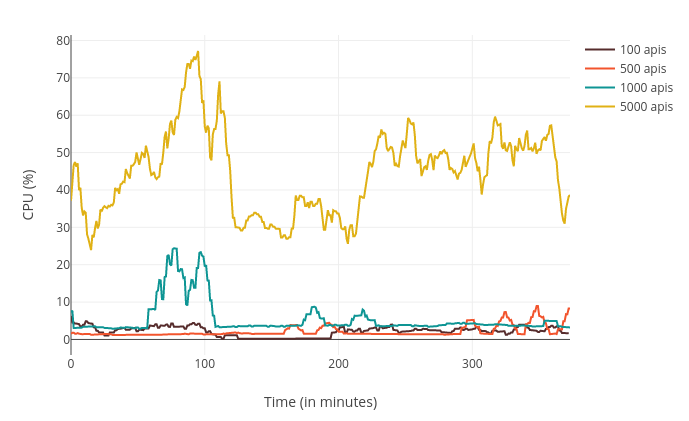
\includegraphics[width=0.9\textwidth]{./images/chapter5/cpu-plot.png}
	\caption[Αποτελέσματα χρήσης της CPU.]{Αποτελέσματα χρήσης της CPU.}
	\label{fig:cpu_usage}
\end{figure}

\begin{figure}[H]
	\centering
	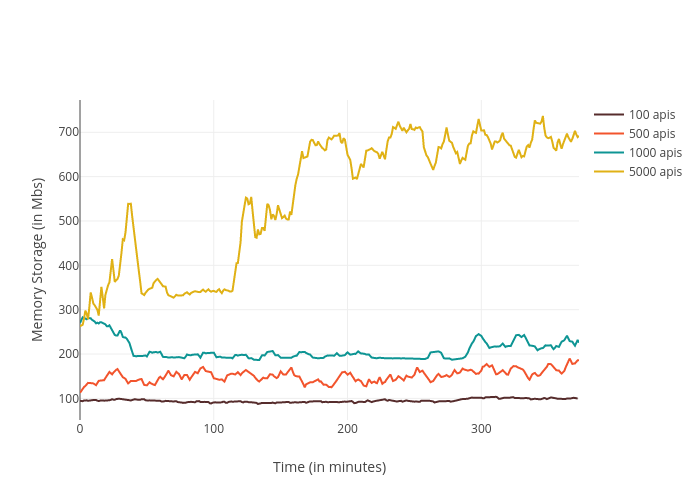
\includegraphics[width=0.9\textwidth]{./images/chapter5/memory-plot.png}
	\caption[Αποτελέσματα χρήσης της RAM]{Αποτελέσματα χρήσης της RAM}
	\label{fig:ram_usage}
\end{figure}

\clearpage

\section{Επίδειξη Εφαρμογής}
\label{section:webapp_showcase}

Στη συνέχεια παρατίθενται εικόνες από τη χρήση της γραφικής διεπαφής που υλοποιήσαμε, μέσω της οποίας
οι χρήστες μπορούν να επικοινωνούν με το backend.

Στo \autoref{fig:lychte_overview} μπορούμε να δούμε όλα τα Apis που έχουμε ενεργά, καθώς και κάποια στοιχεία σχετικά με αυτά.
Η πληροφορία που δείχνουμε σε αυτήν την εικόνα, αφορά δεδομένα μέχρι μία ημέρα πριν. Αυτό γίνεται για να δώσουμε αρχικά μία γενική εικόνα
των υπό μελέτη εξωτερικών συστημάτων, αλλά και να περιορίσουμε το πλήθος της πληροφορίας που θα πρέπει να ληφθεί υπόψη,
ώστε να μπορεί να ανταποκρίνεται πιο γρήγορα και να είναι έτσι πιο αποδοτικά τα queries που κάνουμε στη βάση δεδομένων μας. Μερικά από
τα στοιχεία που παρουσιάζονται αφορούν το πλήθος των ελέγχων που πραγματοποιήθηκαν εντός των τελευταίων εικοσιτεσσάρων ωρών, η μέση διάρκεια και η τυπική
απόκλιση των αποκρίσεων των αιτημάτων που κάναμε, ο μέσος βαθμός επιτυχών αποκρίσεων και η κατάσταση του τελευταίου αποθηκευμένου ελέγχου. \\
\\

\begin{figure}[!ht]
	\centering
	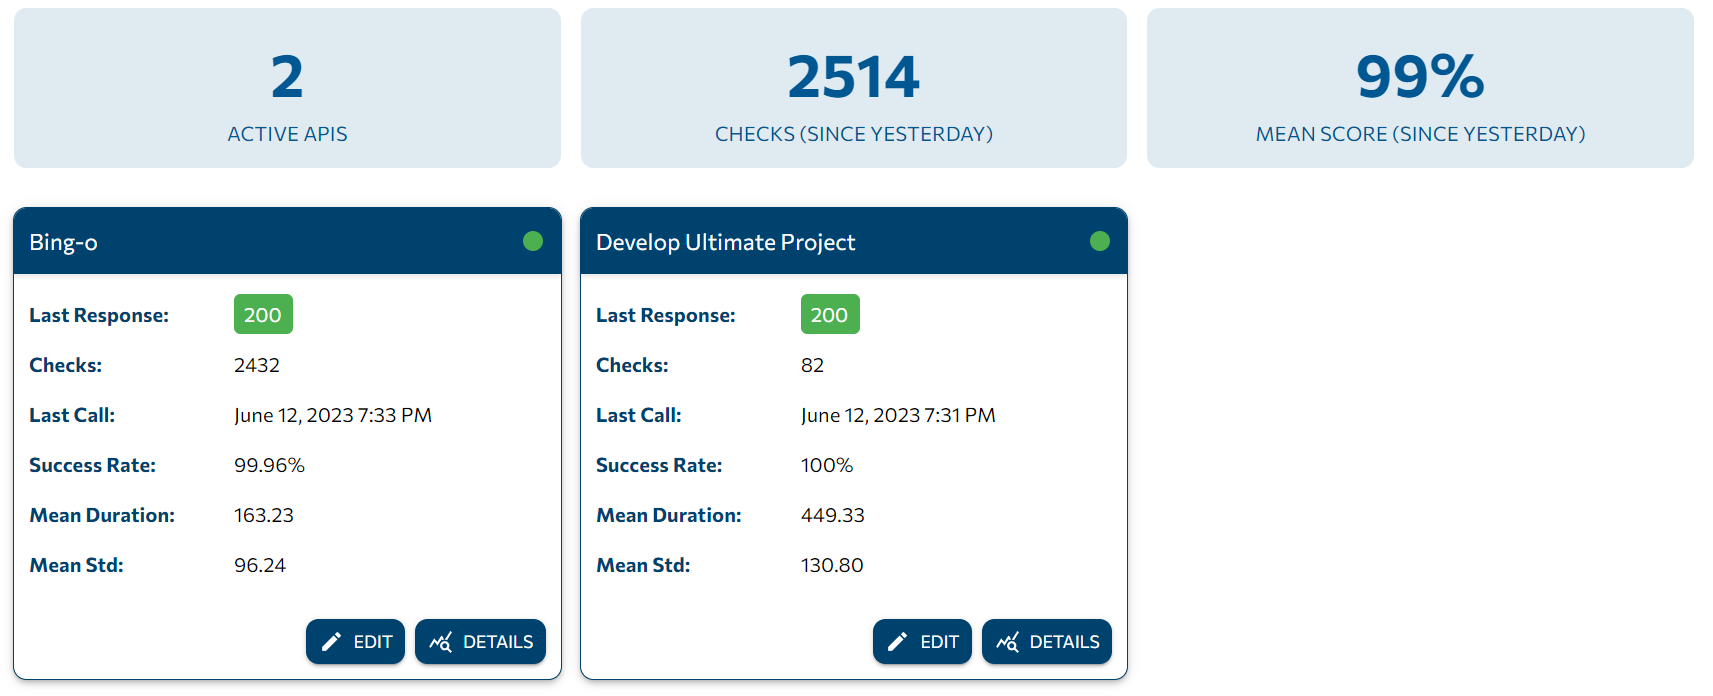
\includegraphics[width=1\textwidth]{./images/chapter5/overview_landing.png}
	\caption[Lychte Api Overview]{Lychte Api Overview}
	\label{fig:lychte_overview}
\end{figure}

\clearpage

Έπειτα στα \cref{fig:lychte_create_api,fig:lychte_advanced_api_creation}, φαίνονται
τα στοιχεία που καλείται να συμπληρώσει η χρήστης για να φτιάξει κάποιο καινούργιο Api στο σύστημά μας και να ξεκινήσουν
οι έλεγχοι. \\

\begin{figure}[!ht]
	\centering
	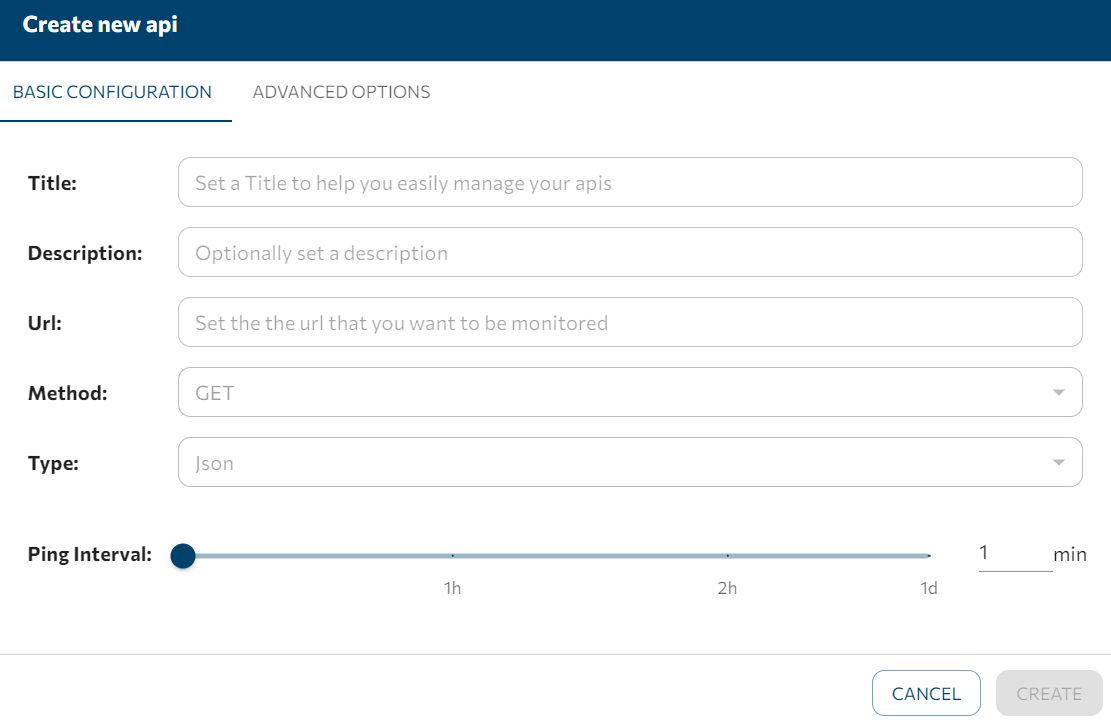
\includegraphics[width=0.8\textwidth]{./images/chapter5/api_creation.png}
	\caption[Εικόνα Βασικών Στοιχείων προς συμπλήρωση από το χρήση]{Εικόνα Βασικών Στοιχείων προς συμπλήρωση από το χρήση}
	\label{fig:lychte_create_api}
\end{figure}

\begin{figure}[!ht]
	\centering
	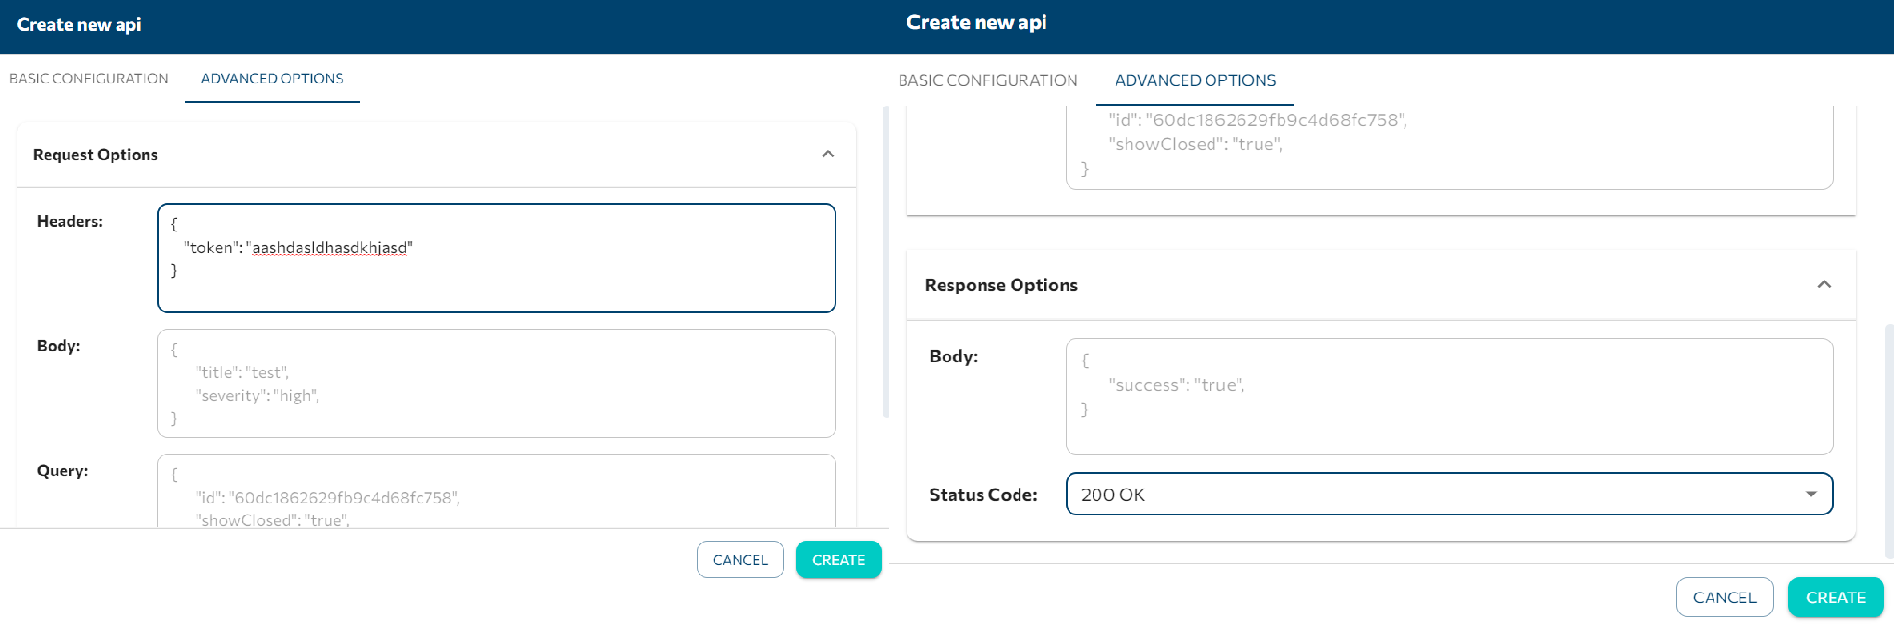
\includegraphics[width=0.9\textwidth]{./images/chapter5/api_creation_advanced.png}
	\caption[Εικόνες Εισαγωγής "Προηγμένων" στοιχείων για τη δημιουργία νέου ελέγχου]{Εικόνες Εισαγωγής "Προηγμένων" στοιχείων για τη δημιουργία νέου ελέγχου}
	\label{fig:lychte_advanced_api_creation}
\end{figure}

\clearpage

Στη συνέχεια, παρουσιάζονται διαγράμματα που μπορεί να δει ο χρήστης και σχετίζονται, όπως και πριν, με δεδομένα
των τελευταίων εικοσιτεσσάρων ωρών. Τα διαγράμματα ανανεώνονται αυτόματα κάθε ένα λεπτό προκειμένου να δείχνουν
πάντα την τελευταία έκδοση των δεδομένων που έχουμε αποθηκευμένα. Στο \autoref{fig:lychte_response_duration_breakdown}
μπορούμε να δούμε το χρόνο που μεσολάβησε από τη στιγμή που γίνεται κάποιο αίτημα μέχρι να ανταποκριθεί το υπό μελέτη
σύστημα, σε βάθος χρόνου ημέρας, μπορούμε, ωστόσο, να επιλέξουμε αν θελουμε να φιλτράρουμε τα δεδομένα στις τελευταίες τρεις, έξι και δώδεκα ώρες.
Με μία διακεκομμένη γραμμή αναπαριστούμε το μέσο ώρο του χρόνου που μετρήσαμε. Τέλος, όσον αφορά, τα δεδομένα της τελευταίας μέρας
υπάρχει και το ραβδόγραμμα που φαίνεται στο \autoref{fig:lychte_succesfull_responses}, στο οποίο μπορούμε να δούμε την κατάσταση των τελευταίων
πενήντα αποκρίσεων.\\

\begin{figure}[!ht]
	\centering
	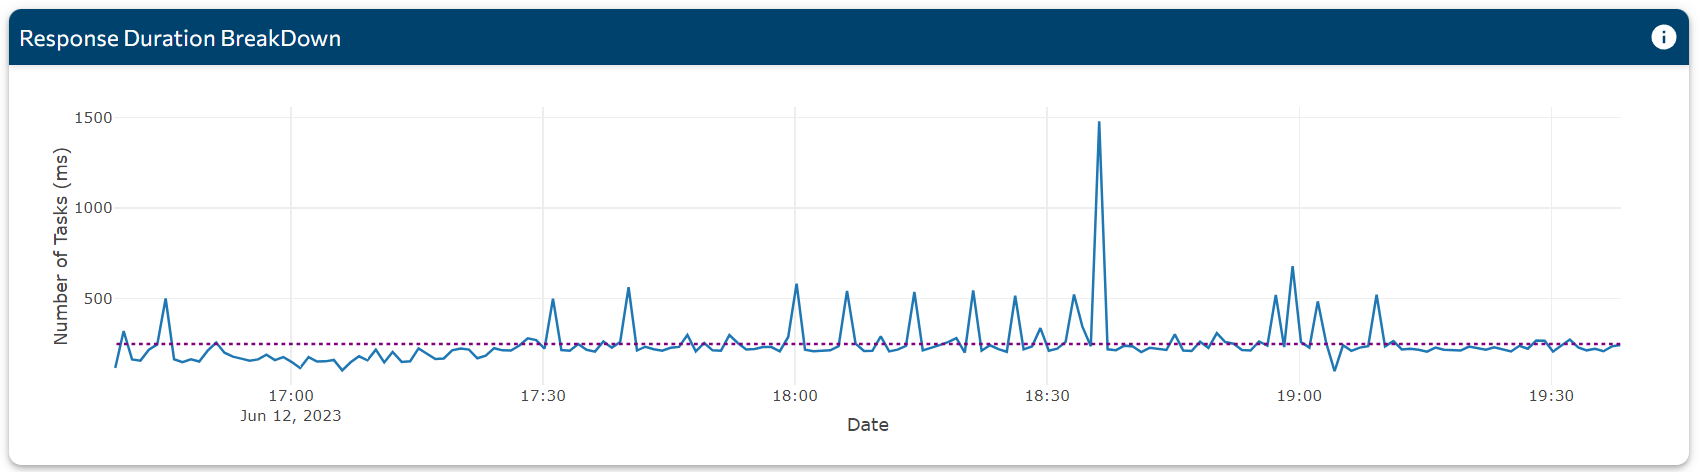
\includegraphics[width=0.9\textwidth]{./images/chapter5/response_duration_breakdown.png}
	\caption[Διάγραμμα Διάρκειας Αποκρίσεων]{Διάγραμμα Διάρκειας Αποκρίσεων}
	\label{fig:lychte_response_duration_breakdown}
\end{figure}	
\begin{figure}[!ht]
	\centering
	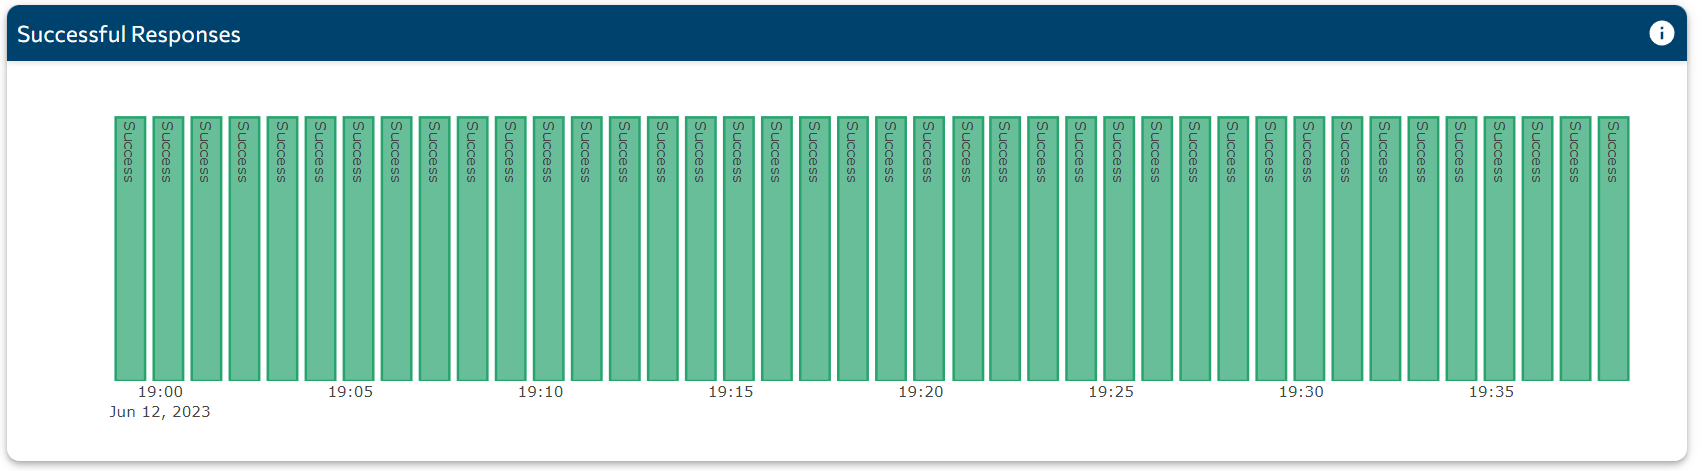
\includegraphics[width=0.9\textwidth]{./images/chapter5/succesfull_responses.png}
	\caption[Ραβδόγραμμα Κατάστασης Αποκρίσεων]{Ραβδόγραμμα Κατάστασης Αποκρίσεων}
	\label{fig:lychte_succesfull_responses}
\end{figure}

Tέλος, θα δείξουμε διαγράμματα και μετρικές που προκύπτουν από το σύνολο των δεδομένων που υπάρχουν
τόσο στη Mongo βάση υπό μορφή documents, όσο και στη Google Cloud βάση, υπό τη μορφή αρχείων. Πιο συγκεκριμένα, αξιοποιούμε
τα ήδη υπολογισμένα δεδομένα που υπάρχουν σε αρχεία τις μορφής \textbf{"/:apiId/stati\hyp{}stics.avro"}. Στα
δεδομένα που αντλούμε από τα προαναφερθέντα αρχεία, ενσωματώνουμε όσα δεν έχουν αποθηκευτεί ακόμα εκεί και βρίσκονται
στη MongoDB. Κάθε φορά που γίνονται οι υπολογισμοί αυτοί, και για να γλιτώσουμε τέτοιους συνεχείς
υπολογισμούς, αποθηκεύουμε όσα στοιχεία χρειαζόμαστε σε μία νέα συλλογή δεδομένων στην κύρια βάση μας (ονομασία \textbf{Statistics}), που αποθηκεύει
στατιστικά. Κάθε φορά που φορτώνει η συγκεκριμένη σελίδα, ελέγχει αν υπάρχει καταχώρηση για το συγκεκριμένο Api στο νέο αυτό collection εντός
ενός χρονικού διαστήματος (τριάντα λεπτών). Αν υπάρχει, αντλεί τα δεδομένα από εκεί. Αλλιώς, κάνει τους απαραίτητους υπολογισμούς και στο τέλος
αποθηκεύει τα αποτελέσματα εκεί, με αποτέλεσμα τα επόμενα, χρονικά κοντινά, αιτήματα να ικανοποιούνται πιο γρήγορα.

Στα \cref{fig:lychte_metrics,fig:lychte_boxplot} παρουσιάζονται μετρικές που υπολογίζονται στο σύνολο των ιστορικών δεδομένων
και ένα διάγραμμα Θηκογραμμάτων της διάρκειας απόκρισης των ελέγχων που πραγματοποιήθηκαν, ομαδοποιημένα σε διαστήματα ημέρας.   

\begin{figure}[!ht]
	\centering
	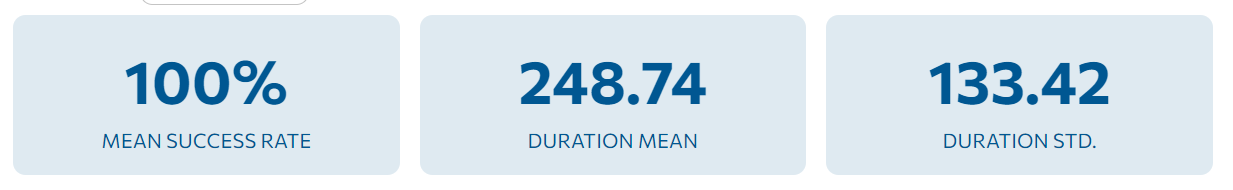
\includegraphics[width=0.8\textwidth]{./images/chapter5/metrics.png}
	\caption[Μετρικές που αφορούν το σύνολο των δεδομένων (ιστορικά δεδομένα)]{Μετρικές που αφορούν το σύνολο των δεδομένων (ιστορικά δεδομένα)}
	\label{fig:lychte_metrics}
\end{figure}

\begin{figure}[!ht]
	\centering
	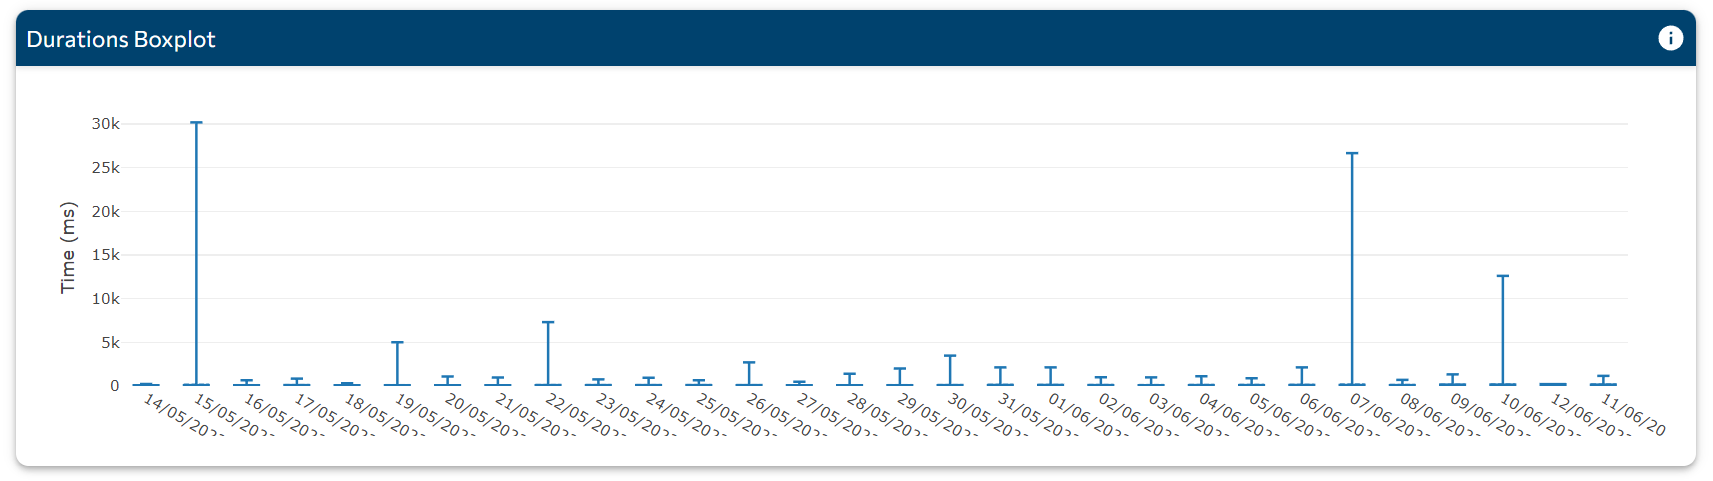
\includegraphics[width=0.9\textwidth]{./images/chapter5/duration_boxplot_diagram.png}
	\caption[Διάγραμμα Θηκογραμμάτων (Boxplots) της διάρκειας απόκρισης αιτημάτων για κάθε μέρα (ιστορικά δεδομένα)]{Διάγραμμα Θηκογραμμάτων (Boxplots) της διάρκειας απόκρισης αιτημάτων για κάθε μέρα (ιστορικά δεδομένα)}
	\label{fig:lychte_boxplot}
\end{figure}
